
In den vorangegangenen Kapiteln wurde gezeigt, wie innerhalb der Web- und 
Service-Schicht testgetrieben entwickelt werden kann. Dabei wurde zunächst die 
Benutzeroberfläche entwickelt und damit verbunden auch die Web-Steuereinheiten -- 
die Controller. Diese rufen unter anderem die für die Benutzeranfragen zuständigen 
Service-Methoden auf. Die einzelnen Services verwenden wiederum geeignete 
Repository-Interfaces und ihre Methoden als Schnittstelle zur Persistenzschicht, deren 
konkrete Implementierungen für das Laden der entsprechenden Daten aus der Datenbank 
verantwortlich sind. Das folgende Kapitel soll sich demnach der testgetriebenen 
Entwicklung dieser Repositories -- und damit verbunden der Persistenzschicht im 
Allgemeinen -- widmen. \\ 
Im Allgemeinen ist zu sagen, dass für sämtliche Datenbank-Tests die 
\texttt{Testcontainers}-Bibliothek in Kombination mit \texttt{Docker} verwendet wird. 
Eine solche Konfiguration bietet gleich mehrere Vorteile: Erstens werden so 
realistische Tests mit einer echten Instanz der für das Projekt ausgewählten 
Datenbank ermöglicht. Die Test-Datenbank kann somit exakt so wie die 
Produktiv-Datenbank konfiguriert werden, wodurch möglichst realistische Bedingungen 
simuliert werden. \\ 
Zweitens sorgt die Verwendung von \texttt{Testcontainers} dafür, dass jeder Test in 
einer bereinigten Umgebung stattfindet, um zu verhindern, dass sie einander 
beeinflussen und das Ergebnis verfälschen. Drittens wird das Hoch- und Runterfahren 
sowie das Setup des \texttt{Docker-Containers} automatisiert und von 
\texttt{Testcontainers} übernommen. \\ 
Doch um \texttt{Testcontainers} mit seinen zuvor benannten Vorteilen nutzen zu können, 
muss auch ein gewisser Preis gezahlt werden, denn mit der Verwendung der Java-Bibliothek 
gehen wiederum auch einige Nachteile einher. Die realistischen Tests mit einer 
Test-Datenbank benötigen zusätzliche Systemressourcen und das Starten sowie Stoppen der
Test-Container benötigt Zeit, besonders dann, wenn Images gezogen werden müssen. 
Außerdem benötigt \texttt{Testcontainers} eine funktionierende Docker-Installation, was 
wiederum eine weitere Abhängigkeit darstellt. \\ 
Daher muss bei der Konzeption der Datenbank-Tests stets abgewogen werden, ob nun die 
Vor- oder Nachteile überwiegen und damit verbunden die spezifischen Anforderungen des 
jeweiligen Projektes geprüft werden, um schließlich die bestmögliche Lösung zu wählen. 
Im Falle des Spielzeitenplaners überwiegen die zuvor beschriebenen Vorteile, denn es 
soll Wert auf realitätsnahe Datenbank-Tests gelegt werden, Nachteile wie der erhöhte 
Ressourcenbedarf oder die längeren Testlaufzeiten haben hier keine große Relevanz. \\ 
Grundsätzlich sind alle Datenbank-Testklassen, die im Verzeichnis 
\href{https://github.com/FlorianOhmes/bat_spielzeitenplaner/tree/main/spielzeitenplaner/src/test/java/de/bathesis/spielzeitenplaner/database}{\texttt{src/test/java/de \linebreak /bathesis/spielzeitenplaner/database}}
zu finden sind, auf die gleiche Art und Weise aufgebaut. Zunächst einmal muss die 
jeweilige Testklasse mit drei verschiedenen Annotationen versehen werden: 
(1.) \texttt{@DataJdbcTest}, durch die Spring eine spezielle Testumgebung für die 
Persistenzschicht konfiguriert -- der Web-Layer zum Beispiel wird komplett deaktiviert 
-- um ressourcenschonender arbeiten zu können, (2.) 
\texttt{@AutoConfigureTestDatabase(replace = AutoConfigureTestDatabase.Replace.NONE)}, 
die dafür sorgt, dass Spring die Produktiv-Datenbank nicht automatisch durch eine 
\texttt{In-Memory}-Datenbank ersetzt, sondern die durch \texttt{Testcontainers} 
konfigurierte Test-Datenbank benutzt, und (3.) \texttt{@Testcontainers}, die für die 
Verwaltung der innerhalb der Klasse definierten Container zuständig ist 
(\texttt{Start}, \texttt{Stop} und \texttt{CleanUp}). \\ 
In dem nun folgenden Schritt wird ein solcher Container definiert. Dies geschieht 
durch folgendes Statement: 

\begin{quote}
\begin{verbatim}
@Container
private static PostgreSQLContainer<?> postgresContainer = 
        new PostgreSQLContainer<>("postgres:15-alpine")
                .withDatabaseName("testdb")
                .withUsername("testuser")
                .withPassword("testpassword");
\end{verbatim}
\end{quote}

Es wird ein \texttt{Postgres}-Container erstellt und konfiguriert, indem die 
\texttt{PostgreSQL}-Version, der Name der Test-Datenbank sowie Benutzername und 
Passwort festgelegt werden. Auch weitere Konfigurationsmöglichkeiten können hier 
hinzugefügt werden, um die Datenbank den Ansprüchen entsprechend zu gestalten. Die 
\texttt{@Container}-Annotation sorgt dafür, dass der \texttt{Postgres}-Container 
als solcher erkannt wird und das zuvor erwähnte Starten und Stoppen automatisiert 
werden kann. \\ 
Damit \texttt{Spring} sich nun auch wirklich mit der Test-Datenbank -- und nicht mit 
der Produktiv-Datenbank -- verbindet, müssen die Eigenschaften der ursprünglichen 
Datenbankverbindung, die in der \texttt{application.yaml} festgelegt sind, während 
der Tests überschrieben werden. Dies geschieht mithilfe der mit 
\texttt{@DynamicPropertySource}-annotierten \texttt{configureProperties}-Methode. 
Innerhalb dieser werden in der \texttt{DynamicPropertyRegistry} die nötigen 
Verbindungseigenschaften -- darunter die dynamisch generierte \texttt{JdbcUrl} sowie 
\texttt{Username} und \texttt{Password} der durch den \texttt{postgreSQLContainer} 
definierten Test-Datenbank -- festgelegt. Ist dies geschehen, so wird die 
Produktiv-Datenbank für die Dauer der Tests erfolgreich durch die Test-Datenbank 
substituiert. \\ 
Bevor nun konkret mit dem Schreiben einzelner Tests begonnen werden kann, müssen 
die notwendigen Repositories bereitgestellt werden. Da eine strikte Einhaltung der 
Onion-Architektur klar definierte Schnittstellen zwischen der inneren Schicht der 
Domäne und äußeren Schichten -- wie der Persistenzschicht -- erfordert, müssen diese 
bereits bei der Entwicklung der Service-Schicht definiert werden. Auch das in den Tests 
verwendete Mocking ist ohne die Existenz der Klasse gar nicht möglich. Im gleichen Zuge 
ist dann auch direkt eine Klasse für die jeweilige Repository-Implementierung erstellt 
worden, auch wenn diese bis zu diesem Zeitpunkt noch leer bleibt. Lediglich die 
\texttt{@Repository}-Annotation muss verwendet werden, da sonst der
\texttt{contextLoads()}-Test fehlschlägt, weil Spring die relevante \texttt{Bean} nicht 
finden kann. \\ 
Zur Veranschaulichung dieses Sachverhalts soll nun die 
\href{https://github.com/FlorianOhmes/bat_spielzeitenplaner/blob/main/spielzeitenplaner/src/test/java/de/bathesis/spielzeitenplaner/database/DatabaseAssessmentTest.java}{\texttt{DatabaseAssessmentTest.java}}
\linebreak dienen. 
Konkret auf die \texttt{Assessment-Repositories} bezogen ergeben sich folgende \linebreak 
\href{https://github.com/FlorianOhmes/bat_spielzeitenplaner/blob/fccaa502124b53ec672754dc262bb2d6ad1cd867/spielzeitenplaner/src/main/java/de/bathesis/spielzeitenplaner/services/repos/AssessmentRepository.java}{\texttt{AssessmentRepository.java}} 
und 
\href{https://github.com/FlorianOhmes/bat_spielzeitenplaner/blob/fccaa502124b53ec672754dc262bb2d6ad1cd867/spielzeitenplaner/src/main/java/de/bathesis/spielzeitenplaner/database/repoimpl/AssessmentRepositoryImpl.java}{\texttt{AssessmentRepositoryImpl.java}}, 
wie den verknüpften Links zu entnehmen ist. 

\pagebreak

Nun muss ein 
\href{https://github.com/FlorianOhmes/bat_spielzeitenplaner/blob/0a423a3298919d7206b87d381ecbbd66c6c54869/spielzeitenplaner/src/main/java/de/bathesis/spielzeitenplaner/database/springrepos/SpringDataAssessmentRepository.java}{\texttt{SpringDataAssessmentRepository}} 
-- kurz: \texttt{SpringRepository} -- erstellt werden, das wiederum ein 
\texttt{Interface} ist und gewissermaßen eine Brücke zwischen der Anwendung und 
der Datenbank bildet. Es erbt von \texttt{CrudRepository} und ermöglicht die 
sogenannten \texttt{CRUD-Operationen} -- also \texttt{Create}, \texttt{Read}, 
\texttt{Update} und \texttt{Delete} -- bezogen auf die Entität \texttt{Assessment}. 
Dieses \texttt{SpringRepository} wird dann mithilfe der 
\texttt{@Autowired}-Annotation und eines Konstruktors in der 
\texttt{DatabaseAssessmentTest.java} in das \texttt{AssessmentRepository} injiziert. 
Dieses Vorgehen erfordert wiederum einen Konstruktor in der 
\texttt{Assessment \linebreak RepositoryImpl.java}, der zu diesem Zeitpunkt erstellt 
werden kann. \\ 
Um die Persistenzschicht und ihre Daten klar von den anderen Schichten abzutrennen, 
verwendet das \texttt{SpringRepository} eine eigene \texttt{Assessment}-Klasse, die 
im Verzeichnis
\href{https://github.com/FlorianOhmes/bat_spielzeitenplaner/tree/main/spielzeitenplaner/src/main/java/de/bathesis/spielzeitenplaner/database/entities}{\texttt{src/main/java/de/bathesis/spielzeitenplaner/database/entities}}
verortet ist. Sie kann zunächst als einfacher \texttt{Record} mit den entsprechenden 
Attributen aus der Domain-Klasse implementiert werden. Zur Verdeutlichung der zuvor 
beschriebenen Schritte sowie der Trennung der Service- und Persistenzschicht und ihre 
Schnittstellen kann Abbildung 5 herangezogen werden. \\ 

\begin{figure}[h]
  \centering
  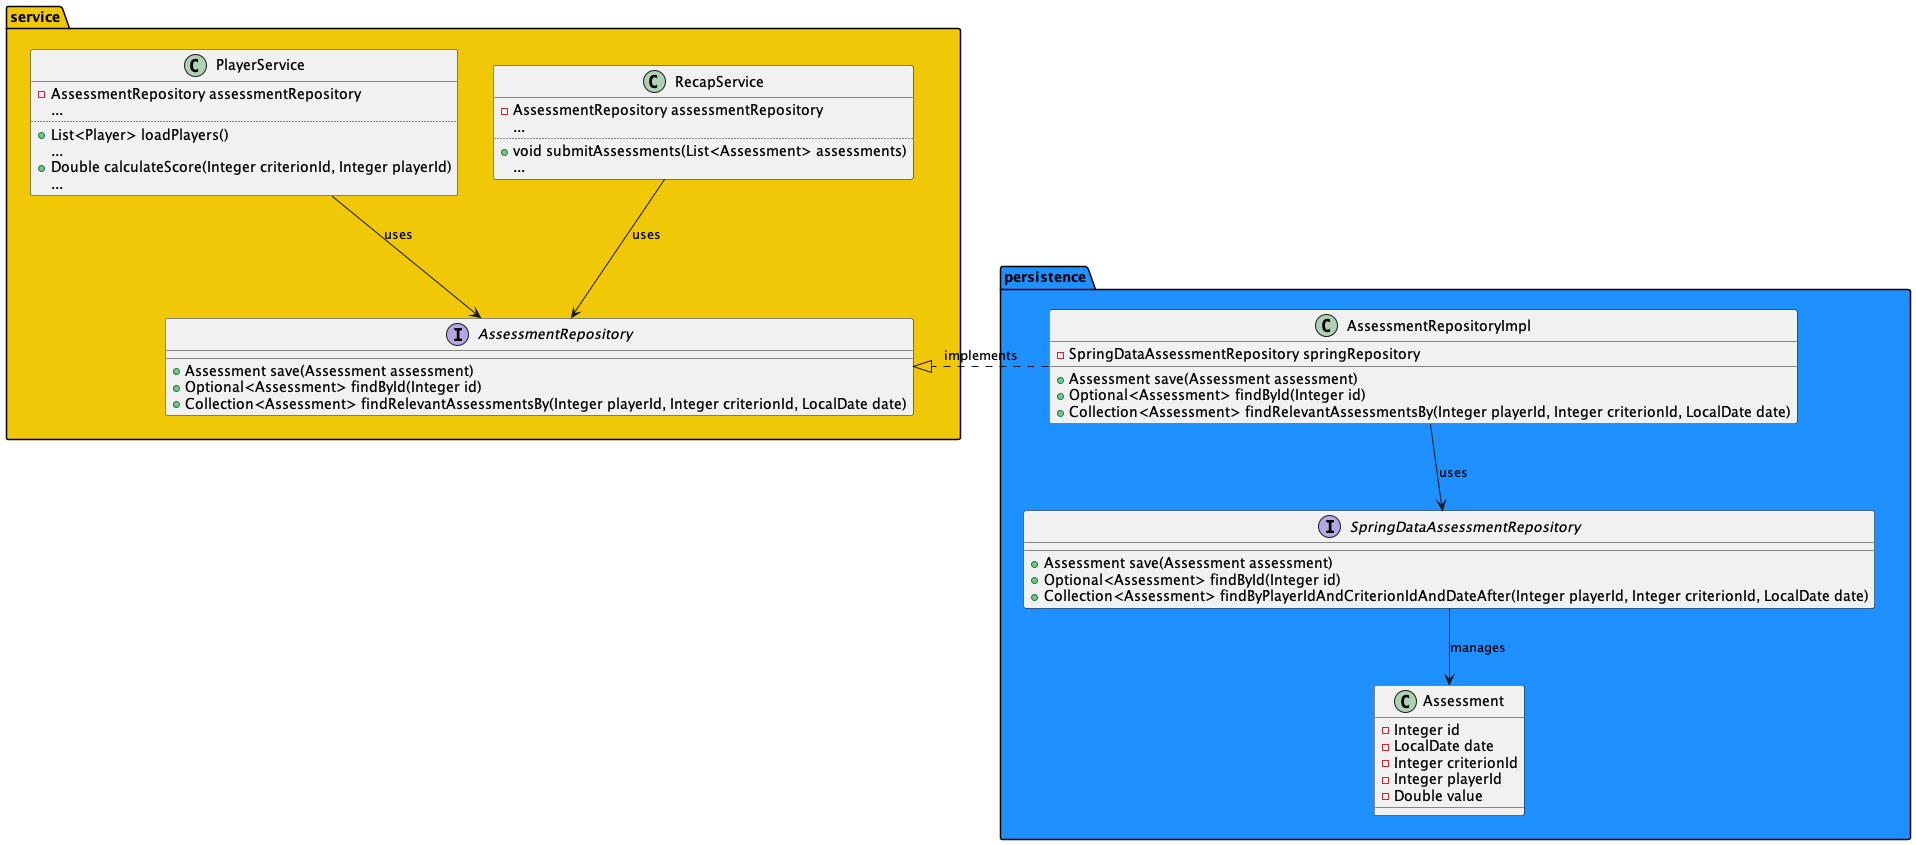
\includegraphics[width=\textwidth]{screenshots/persistence.png}
  \caption{Modellierung von Service- und Persistenzschicht am Beispiel der Assessment.java}
  \label{fig:persistence}
\end{figure}

Sind all die zuvor beschriebenen Schritte vollzogen, so kann mit dem Schreiben 
konkreter Tests begonnen werden. Zunächst einmal ist es wichtig, dass das Speichern 
und Laden einer Entität wie gewünscht funktioniert. Diese beiden Operationen sind 
untrennbar miteinander verbunden, denn um zu überprüfen, ob eine Entität korrekt in 
der Datenbank gespeichert wurde, muss diese zunächst geladen werden. Gleiches gilt für 
Umkehrrichtung: Um zu überprüfen, ob eine Entität korrekt geladen wurde, muss diese 
zunächst in die Datenbank eingefügt werden. Der Test, der feststellt, ob eine 
Bewertung korrekt gespeichert und geladen wird, kann wie folgt geschrieben werden: 

\pagebreak

\begin{quote}
\begin{verbatim}
@Test
void test_01() {
    Assessment assessment = new Assessment(
        null, LocalDate.of(2022, 12, 31), 1, 1, 3.0
    );

    Assessment saved = assessmentRepository.save(assessment);
    Assessment loaded = assessmentRepository
        .findById(saved.getId()).get();

    assertThat(loaded).isEqualTo(saved);
}
\end{verbatim}
\end{quote}

Zuerst wird ein zu speicherndes Test-Objekt erstellt. Dieses wird dann mittels der 
\texttt{save}-Methode in der Datenbank gespeichert und mit \texttt{findById} geladen, 
ehe das gespeicherte mit dem geladenen Objekt abgeglichen und auf Gleichheit geprüft 
wird. Damit dieser Test nun bestehen kann, muss die \texttt{Docker}-Anwendung -- 
das hier zur Entwicklung genutzte Endgerät verwendet die \texttt{Docker Desktop-App} -- 
auf dem testenden Gerät laufen. Darüber hinaus können dem 
\texttt{SpringDataAssessmentRepository} die entsprechenden Methodensignaturen -- 
gemeint sind \texttt{Assessment save(Assessment assessment)} und 
\texttt{Optional<Assessment> findById(Integer id)} -- hinzugefügt werden, um größere 
Kontrolle über deren Implementierung zu erhalten. Dieser Schritt ist in diesem Fall 
jedoch nicht zwingend notwendig, da die Methoden bereits über das 
\texttt{CRUD}-Repository zur Verfügung gestellt werden. \\ 
Schließlich müssen dann auch die im Test genutzten Repository-Mehoden zum Speichern 
und Laden einer Bewertung implementiert werden. Dies gestaltet sich wie folgt: Im 
Falle der \texttt{save}-Methode erfolgt eine Übersetzung des \texttt{DomainAssessment} 
zum \texttt{DatabaseAssessment}, das dann der \texttt{save}-Methode des 
\texttt{SpringDataAssessmentRepository} zum Speichern übergeben werden kann. 
Anschließend wird das gespeicherte Objekt für die Rückgabe vorbereitet, indem es 
zurück in ein entsprechendes Domänen-Objekt konvertiert wird. Der 
\texttt{AssessmentMapper} bzw. die für diese Konvertierung zuständigen Methoden 
müssen an dieser Stelle ebenfalls implementiert werden. Analog dazu wird die 
\texttt{findById}-Methode implementiert, indem die Anfrage an die 
\texttt{findById}-Methode des \texttt{SpringDataAssessmentRepository} delegiert wird 
und dessen Rückgabe zum Domain-Objekt konvertiert und zurückgegeben wird. \\ 
Außerdem sollte sichergestellt werden, dass die entsprechende Tabelle in der Datenbank 
existiert. Ist dies nicht der Fall, wird eine \texttt{BadSqlGrammarException} geworfen, 
da \texttt{JDBC} versucht, die Entität zur Datenbank hinzuzufügen, die entsprechende 
Relation jedoch nicht existiert. Dieser \texttt{Exception} kann beispielsweise 
entgegengewirkt werden, indem mithilfe von \texttt{Flyway} ein entsprechendes 
Migrationsschema erstellt wird. Dazu sollte die Anwendung nach Erstellung des 
Migrationsschemas wenigstens einmal gestartet werden, sodass \texttt{Flyway} die 
Migration durchführen kann. \\ 
Schließlich muss der Instanzvariable \texttt{id} der 
\texttt{Assessment.java} -- gemeint ist die \linebreak \texttt{DatabaseAssessment}-Klasse 
im Verzeichnis \texttt{database/entities} -- noch die \texttt{@Id}-Annotation hinzugefügt 
werden, damit \texttt{JDBC} weiß, dass es sich hierbei um dem Primärschlüssel der 
Tabelle handelt und Anfragen somit ordnungsgemäß ausführen kann. \\ 
Neben \texttt{save} und \texttt{findById} stellt die \texttt{findAll}-Methode 
ebenfalls ein nützliches Werkzeug zum Laden mehrerer Entitäten aus der Datenbank dar, 
das im Rahmen des Spielzeitenplaners häufig Gebrauch findet. Der Ablauf des Tests 
ist dem der \texttt{findById}-Methode ähnlich und ist zum Beispiel unter dem Namen 
\texttt{test\_02} in der
\href{https://github.com/FlorianOhmes/bat_spielzeitenplaner/blob/main/spielzeitenplaner/src/test/java/de/bathesis/spielzeitenplaner/database/DatabasePlayerTest.java}{\texttt{DatabasePlayerTest.java}}
zu finden. Dort werden zunächst mehrere Spieler gespeichert und anschließend 
mithilfe der \texttt{findAll()}-Methode des \texttt{CRUD}-Repositories geladen. 
Abschließend wird dann geprüft, ob die zuvor gespeicherten Elemente durch die 
\texttt{findAll}-Methode gefunden werden. \\ 
Dank \texttt{JDBCs} \texttt{Derived Queries} ist es möglich, über die standardmäßig 
implementierten Basismethoden hinaus auch eigene, spezifischere Methoden zu schreiben, 
die anhand des Methodennamens sowie aufgrund bestimmter Regeln und Konventionen 
entsprechende Anfragen ableiten und ausführen können. Im Kontext des 
Spiezeitenplaners beispielsweise ist es für die Berechnung der Scores hilfreich, 
die gespeicherten Bewertungen nach mehreren Kriterien -- wie dem Namen, Kriterium 
und Datum -- zu filtern, sodass die Score-Berechnung auch nur die gewünschten Daten 
als Grundlage nimmt. Ein 
\href{https://github.com/FlorianOhmes/bat_spielzeitenplaner/blob/main/spielzeitenplaner/src/test/java/de/bathesis/spielzeitenplaner/database/DatabaseAssessmentTest.java}{\texttt{Test}} 
für die so entstandene \texttt{findRelevantAssessmentsBy}-Methode kann 
wie folgt aussehen: 

\begin{quote}
\begin{verbatim}
@Test
...
void test_02() {
    Integer playerId = 1;
    Integer criterionId = 1;
    Assessment assessment1 = new Assessment(
        null, LocalDate.of(2022, 12, 31), criterionId, playerId, 5.0
    );
    Assessment assessment2 = new Assessment(
        null, LocalDate.of(2022, 12, 29), criterionId, playerId, 3.0
    );
    Assessment assessment3 = new Assessment(
        null, LocalDate.of(2022, 12, 31), criterionId, 2, 2.0
    );
    Assessment saved1 = assessmentRepository.save(assessment1);
    Assessment saved2 = assessmentRepository.save(assessment2);
    Assessment saved3 = assessmentRepository.save(assessment3);

    Collection<Assessment> found = 
        assessmentRepository.findRelevantAssessmentsBy(
            playerId, criterionId, LocalDate.of(2022, 12, 1)
    );

    assertThat(found).containsExactly(saved1, saved2);
    assertThat(found).doesNotContain(saved3);
}
\end{verbatim}
\end{quote}

Auch in diesem Fall ist es zunächst notwendig einige Vorbereitungen zu treffen: 
Benötigte sowie geeignete Test-Daten müssen generiert und in der Datenbank gespeichert 
werden, ehe diese dann in einem \texttt{Act}-Schritt abgerufen und gefiltert 
werden. Ob dieser Schritt wie erwartet funktioniert, wird schließlich überprüft: Im 
Falle des zuvor vorgestellten Tests sollten nur \texttt{assessment1} und 
\texttt{assessment2} bzw. \texttt{saved1} und \texttt{saved2} gefunden werden, 
\texttt{assessment3} bzw. \texttt{saved3} hingegen nicht, da diese Bewertung eine 
andere als die gewünschte \texttt{playerId} besitzt. \\ 
Nach diesem Prinzip kann die Methode unter weiteren, verschiedenen Bedingungen 
getestet werden, um diese robuster zu machen. Zum Beispiel können die 
\texttt{Assessments} so gewählt werden, dass sie überprüfen, ob das Filtern nach 
Datum korrekt funktioniert. Gleiches gilt für das Filtern nach Kriterium. Des Weiteren 
ist auch die Überprüfung von Randfällen sinnvoll, um sicherzustellen, dass die 
Methode auch unter weniger optimalen Bedingungen das richtige Ergebnis liefert. 

